\documentclass{article}
\usepackage[utf8]{inputenc}
\usepackage[english]{babel}
\usepackage{enumerate}
\usepackage{amssymb}
\usepackage{amsthm}
\usepackage{amsmath}
\usepackage{upgreek}
\usepackage[linewidth=0.5pt]{mdframed}

%\usepackage[letterpaper, margin=1.5in]{geometry}

\usepackage{algorithm}
\usepackage{algorithmicx}
\usepackage{algpseudocode}

\relpenalty=10000
\binoppenalty=10000

\usepackage{subcaption} 
 
\addtolength{\jot}{1em} 
\renewcommand{\baselinestretch}{1.15} 
 
\usepackage{listings}
\usepackage{color}

\definecolor{dkgreen}{rgb}{0,0.6,0}
\definecolor{gray}{rgb}{0.5,0.5,0.5}
\definecolor{mauve}{rgb}{0.58,0,0.82}

\usepackage[shortlabels]{enumitem}
\setlist{  
  listparindent=1.5em,
  parsep=0.5em,
}

\lstset{frame=tb,
  language=Python,
  aboveskip=3mm,
  belowskip=3mm,
  showstringspaces=false,
  columns=flexible,
  basicstyle={\small\ttfamily},
  numbers=none,
  numberstyle=\tiny\color{gray},
  keywordstyle=\color{blue},
  commentstyle=\color{dkgreen},
  stringstyle=\color{mauve},
  breaklines=true,
  breakatwhitespace=true,
  tabsize=3
}
 
\usepackage[font=small,labelfont=bf]{caption} 
 
 \usepackage{mathtools}
\usepackage{tikz}
\usepackage{verbatim}
\usepackage[active,tightpage]{preview}
\setlength\PreviewBorder{5pt}% 
\usetikzlibrary{arrows}
 
\newtheorem{theorem}{Theorem}[section]
\newtheorem{corollary}{Corollary}[theorem]
\newtheorem{lemma}[theorem]{Lemma}
\renewcommand\thesubsection{\thesection.\roman{subsection}}

\setlength{\parindent}{0pt}
\setlength{\parskip}{8pt plus 1pt minus 1pt}

\def\hyphen{{\hbox{-}}}
\newcommand{\unit}[1]{\ensuremath{\, \mathrm{#1}}}
\newcommand{\san}[1]{\textsf{#1}}
\newcommand{\p}[1]{\ensuremath{\operatorname{\textsf{P}}\!\left(#1\right)}}
\newcommand{\phat}[1]{\ensuremath{\operatorname{\hat{\textsf{P}}}\!\left(#1\right)}}
\newcommand{\vt}{\,\vert\,}
\newcommand{\call}[2]{\textsc{#1}({#2})}
\newcommand{\ev}{\Big|}
\newcommand{\arr}[1]{\texttt{arr[$#1$]}}
\newcommand{\Var}[1]{\operatorname{Var}(#1)}
\newcommand{\Cov}[1]{\operatorname{Cov}(#1)}
\newcommand{\Corr}[1]{\operatorname{\uprho}(#1)}
\newcommand{\s}{\text{s}}
\newcommand{\overbar}[1]{\mkern 1.5mu\overline{\mkern-2mu#1\mkern-1mu}\mkern 1.5mu}
\newcommand{\pluseq}{\mathrel{+}=}
\newcommand{\asteq}{\mathrel{*}=}

\setlength{\parindent}{4em}

\DeclareMathOperator{\E}{\mathbb{E}}

\DeclarePairedDelimiter\ceil{\lceil}{\rceil}
\DeclarePairedDelimiter\floor{\lfloor}{\rfloor}

\title{The Parallel Paradox}
\author{Andrew Chen (achen28)}

\begin{document}
\maketitle

\setlength{\abovedisplayskip}{1.5em}
\setlength{\belowdisplayskip}{1.5em}
\setlength{\abovedisplayshortskip}{1.5em}
\setlength{\belowdisplayshortskip}{1.5em} 
 

\section{Premise}

Consider a capacitor $C_1$ with capacitance $C$ charged with charge $Q_0$.  An uncharged capacitor $C_2$ also with capacitance $C$ is then added in parallel with a conducting wire.  Because $\Delta V_C = Q / C$, we know that the initial voltage $\Delta V_{C_1}$ over $C_1$ has value $\Delta V_{C_1} = Q_0 / C$.  Additionally, because $C_2$ is initially uncharged, the initial voltage $\Delta V_{C_2}$ over it has value $\Delta V_{C_2} = 0 \unit{C} / C = 0 \unit{V}$.  This difference in voltage results in a voltage gradient along the wires connecting the two capacitors, resulting in current flow $C_1$ to $C_2$.  This current flow continues until the voltage gradient is abolished, which occurs when $\Delta V_{C_1} = \Delta V_{C_2}$, at which time an equilibrium is established.  Because $C_1$ and $C_2$ both have the same capacitance, this can only occur when the charge on $C_1$ is equal to the charge on $C_2$.  Due to conservation of charge, we therefore know that this occurs when $Q_0$ is split evenly across the two capacitors, that is, when each capacitor has charge $Q_0 / 2$.  The initial and post-equilibrium states are graphically shown in Figure 1.

\begin{figure}[h!]
\centering
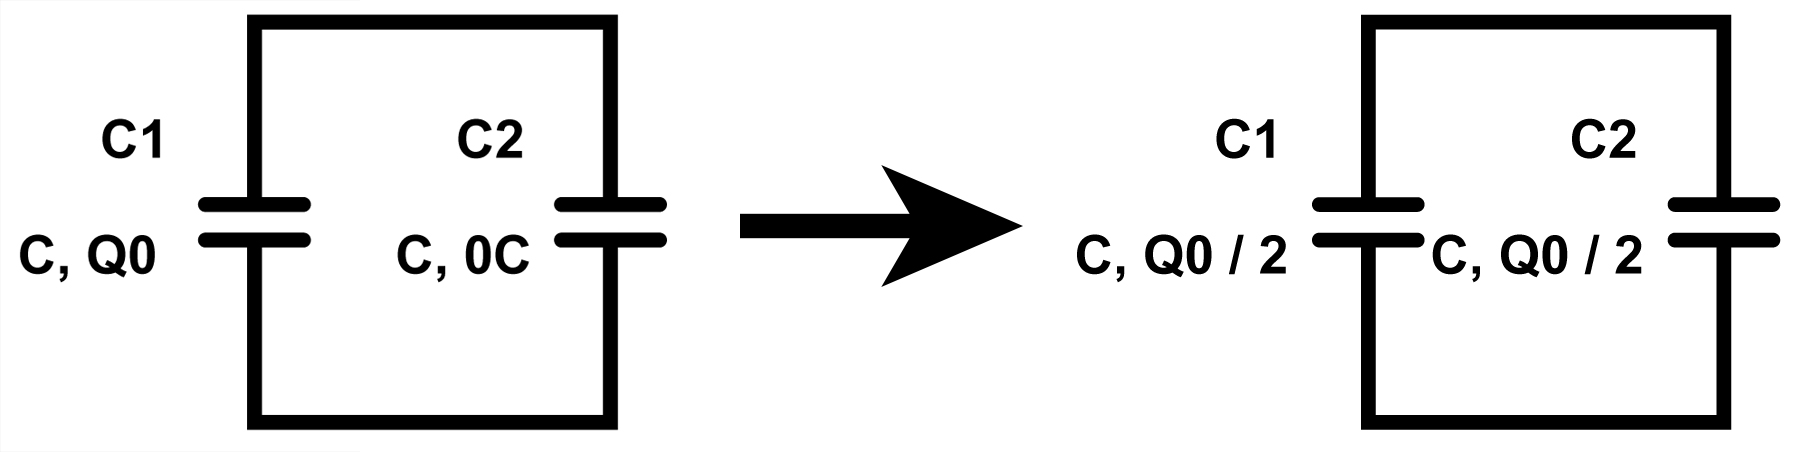
\includegraphics[scale=0.15]{1.jpg} 
\caption{The initial state at the exact time of connection and the equilibrium state, in which there is identical charge on each capacitor.}
\end{figure}

However, recall that the energy $U_C$ stored is a capacitor has a value given by the equation
\[
\frac{1}{2} \frac{Q^2}{C}
\]
In the initial unconnected state, the total energy stored over both capacitors has the following value:
\[
U_{\text{total,i}} = U_{C_1} + U_{C_2} = \frac{1}{2} \frac{Q_0^2}{C} + \frac{1}{2} \frac{(0 \unit{C})^2}{C} = \frac{1}{2} \frac{Q_0^2}{C}
\]
However, at the point of electrostatic equilibrium between the two capacitors after they have been connected in parallel, the total energy stored over both capacitors has a value
\[
U_{\text{total,f}} = U_{C_1} + U_{C_2} = \frac{1}{2} \frac{(Q_0 / 2)^2}{C} + \frac{1}{2} \frac{(Q_0 / 2)^2}{C} =  \frac{Q_0^2 / 4}{C} = \frac{1}{4} \frac{Q_0^2}{C}
\]
We find that $U_{\text{total,f}} = \frac{1}{2}U_{\text{total,i}}$, that half of the energy that was initially stored in the capacitors has disappeared.  Energy must be conserved, so where has this energy gone?

\section{Maybe the Wires Aren't so Ideal}

Typically, in circuit analysis, we consider wires to be ideal conductors with negligible resistance.  This is typically a simplifying assumption that allows for more straightforward reasoning about ideal circuits.  However, in reality, conducting wires typically have a nonnegligible resistance.  Therefore, it might be the case that some of the energy that disappeared was dissipated by the wire.

\begin{figure}[h!]
\centering
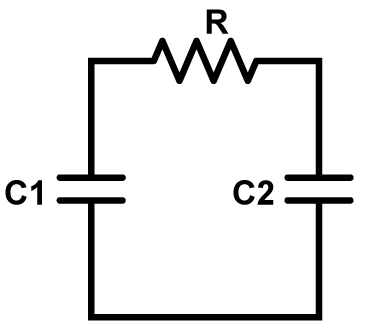
\includegraphics[scale=0.2]{2.png} 
\caption{A new circuit construction where the wires are not ideal and have total resistance $R$.}
\end{figure}

In order to assess this claim, let's assume that the connecting wires have a total resistance $R$ where $R > 0 \unit{\Omega}$ (Figure 2).  Then, we can create the following loop equation:
\[
-IR + \Delta V_{C_1} - \Delta V_{C_2} = 0 \unit{V}
\]
Because $I = -dQ/dt$, where $Q$ is the charge on $C_1$, this equation is equivalent to
\[
\frac{dQ}{dt} + \frac{Q}{RC} - \frac{Q_0 - Q}{RC} = 0 \unit{V}
\]
We can then manipulate this equation in the following manner:
\begin{align*}
\frac{dQ}{dt} + \frac{Q}{RC} - \frac{Q_0 - Q}{RC} &= 0 \unit{V}\\
\frac{dQ}{dt} &= \frac{Q_0 - Q}{RC} - \frac{Q}{RC} \\
\frac{dQ}{dt} &= \frac{Q_0 - 2Q}{RC} \\
\frac{dQ}{Q_0 - 2Q} &= \frac{dt}{RC} \\
\frac{dQ}{2Q - Q_0} &= -\frac{dt}{RC}
\end{align*}
Integrating this equation, and letting $\tau = RC$, we obtain
\begin{align*}
\int_{Q_0}^Q \frac{dQ}{2Q - Q_0} &= \int_0^\infty -\frac{dt}{RC} \\
\left[ \frac{1}{2} \ln (2Q - Q_0) \right]_{Q_0}^Q &= - \frac{t}{\tau} \\
\ln(2Q - Q_0) - \ln(Q_0) &= -\frac{2t}{\tau} \\
\ln\left(\frac{2Q - Q_0}{Q_0}\right) &= -\frac{2t}{\tau} \\
\frac{2Q - Q_0}{Q_0} &= e^{-2t/ \tau}\\
\frac{2Q}{Q_0} - 1 &= e^{-2t/ \tau}\\
\frac{2Q}{Q_0} &= e^{-2t/ \tau} + 1\\
Q &= \frac{1}{2} Q_0 e^{-2t/ \tau} + \frac{Q_0}{2}
\end{align*}
We have thus found a function $Q(t)$ that quantitatively describes the amount of charge on $C_1$ as a function of time.  We can then determine the amount of charge on $C_2$ as a function of time by the difference of $Q_0$ and $Q(t)$.  We can differentiate $Q(t)$ to find the resistor current.
\[
I(t) = -\frac{dQ}{dt} = \frac{Q_0}{RC} e^{-2t/ \tau} = \frac{\Delta V_0}{R} e^{-2t/ \tau}
\]
From this, we can multiply the equation by $R$ to obtain $\Delta V_R(t)$, which is
\[
\Delta V_R(t) = \Delta V_0 e^{-2t/\tau}
\]
We know that the energy dissipated across the resistor is given by
\[
U_R = \int_0^\infty I(t) \Delta V_R(t) dt
\]
Because we now know $I(t)$ and $\Delta V_R(t)$, we can solve for $U_R$ in the following manner:
\begin{align*}
U_R &= \int_0^\infty I(t) \Delta V_R(t) dt \\
&= \int_0^\infty \left( \frac{\Delta V_0}{R} e^{-2t/ \tau} \right) \left( \Delta V_0 e^{-2t/\tau} \right) dt \\
&= \frac{\Delta V_0^2}{R} \int_0^\infty \left( e^{-2t/ \tau} \right)^2 dt \\
&= \frac{\Delta V_0^2}{R} \int_0^\infty e^{-4t/ \tau} dt \\
&= \frac{\Delta V_0^2}{R} \left[ -\frac{1}{4}e^{-4t / \tau} \right]_0^\infty \\
&= \frac{1}{4} CV_0^2
\end{align*}
Wait for a second, the total energy dissipated over the resistor to reach equilibrium is $\frac{1}{4}CV_0^2$, which is exactly equal to $U_{\text{total, f}}$.  In fact, we see that
\[
U_{\text{total,f}} + U_R = \frac{1}{4}CV_0^2 + \frac{1}{4}CV_0^2 = \frac{1}{2}CV_0^2 = U_{\text{total,i}}
\]
Because we evaluated $U_R$ for an arbitrary positive resistance $R$, we see that as long as the connections between $C_1$ and $C_2$ have resistance, half of the energy initially on $C_1$ is dissipated by the connections.  So energy didn't disappear, it just dissipated through the wire!\footnote{Thank goodness we won't have to rewrite the Laws of Thermodynamics!}

\section{Well, What About the Super Cool Wires?\protect\footnote{Yes, I'm trying to make a superconductor joke...}}

It turns out that in certain materials there exists a state called superconductivity in which the material has no electrical resistance when below a certain (very low) temperature.  In Section 2 we explained how the parallel capacitor paradox can be explained by the fact that all of the "disappeared" energy is dissipated through an ohmic wire.  However, this doesn't hold if the wires are actually ideal, because the proof required a connection with non-zero resistance.  If the wires are superconducting, then we need to find an alternate explanation for the apparent loss of energy from the circuit system.

We can use our knowledge of inductors and electromagnetic waves to formulate a high-level hypothesis as to how the parallel capacitor paradox may be addressed for superconducting wires.  Because the capacitors are in parallel, we know that the overall circuit has at least one complete loop (and is not a perfectly straight wire).  This is effectively a 1+ turn solenoid with a (potentially) weird geometry.  Therefore, even though the wires may be superconducting, they will still have some inductance.  Thus, the entire circuit can be modeled as an LC circuit.  The charge that was initially on $C_1$ then begins to oscillate between the capacitors.

To a stationary observer at a point around the circuit, this oscillation effectively functions as a dipole that repeatedly increases and decreases in strength.  As the dipole appears or disappears, the electric fields surrounding the circuit oscillate in a plane.  This changing electric field induces a magnetic field, which itself in turn induces an electric field, and so on.  This results in the generation of an electromagnetic wave.  Over the time that it takes for the capacitors to equilibrate, half of the initial energy present in $C_1$ is lost through these electromagnetic waves.

\end{document}